% Number 610
% UFPM SFriction Friction Tension Vectors Algebra Units 
% Pulling box at angle - min angle?
% JG

% Watermark
\AddToShipoutPicture*{\BackgroundPic}

\addtocounter {ProbNum} {1}

\begin{floatingfigure}[r]{.35\textwidth}
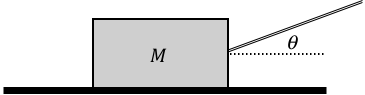
\includegraphics[scale=.6]{/Users/jgates/desktop/latex/pics/pullingbox1}
\end{floatingfigure}
 
{\bf \Large{\arabic{ProbNum}}} A 10 kg box is pulled across the floor by a rope inclined ${21^{\circ}}$ from the horizontal. The coefficient of static friction between the floor and the box is .7 and the coefficient of kinetic friction is .4. 

\bigskip
How hard will the rope need to be pulled in order to set the box in motion?
\paragraph{}
\noindent
\vfill

If the angle is changed, the necessary force to make the box slide changes. Determine the angle at which the tension required to move the box is at a minimum.  You may need to get creative to find that minimum point!
\vfill

%\hfill 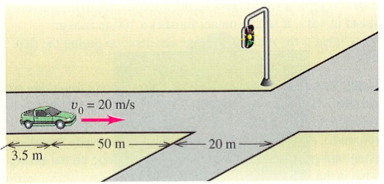
\includegraphics[scale=.85]{/Users/jgates/desktop/latex/pics/redlight.png}
\newpage